\chapter{Metodologia}\label{cap:metodologia}

Este capítulo descreve o ambiente experimental automatizado e o protocolo metodológico desenvolvidos para avaliar a capacidade de LLMs na resolução de problemas do Nível Sênior da OBI, garantindo reprodutibilidade, comparabilidade entre modelos e rigor na verificação das soluções.

\section{Arquitetura Experimental}

A arquitetura experimental foi projetada em estudo anterior~\citep{angelo2026ise} e aprimorada no presente trabalho para automatizar integralmente o ciclo de avaliação em seis blocos funcionais interconectados (\textbf{ENTRY}, \textbf{DATA}, \textbf{ORCHESTRATION}, \textbf{SERVICES}, \textbf{EXTERNAL} e \textbf{OUTPUT}), conforme representado na Figura~\ref{fig:met-arquitetura}. O fluxo inicia-se no ponto de entrada \texttt{main.py} (\textbf{ENTRY}), onde são parametrizados o conjunto de dados em \texttt{database/} (\textbf{DATA}), o modo de execução (oráculo ou geração via LLM), a linguagem de programação (\linguagem{Python}, \linguagem{C}, \linguagem{C++}, \linguagem{Java} ou \linguagem{JavaScript}), o provedor de LLM, o escopo de questões, a modalidade de representação visual (\modalidade{text}, \modalidade{img} ou \modalidade{description}), o modelo de \textit{prompt} e a inclusão opcional dos limites de tempo e memória.

\begin{figure}[!htbp]
\centering
\resizebox{\textwidth}{!}{% Diagrama de arquitetura do sistema de benchmarking (Cap. 4, Seção 4.1)
% Baseado na arquitetura de referência e nos módulos reais em src/
\begin{tikzpicture}[
  x=1cm, y=1cm,
  font=\sffamily\footnotesize,
  panel/.style={draw=black!45, line width=0.8pt, fill=gray!4, rounded corners=2pt},
  panelhdr/.style={draw=black!45, line width=0.8pt, fill=black!75, text=white, font=\sffamily\bfseries\footnotesize, align=center},
  hdrData/.style={panelhdr, fill=vLaranja!85!black},
  hdrEntry/.style={panelhdr, fill=black!75},
  hdrOrch/.style={panelhdr, fill=vAzul!80!black},
  hdrOut/.style={panelhdr, fill=vVerde!80!black},
  hdrSrv/.style={panelhdr, fill=vAzul!85!black},
  hdrExt/.style={panelhdr, fill=black!70},
  boxNode/.style={draw=vAzul!80!black, line width=0.9pt, fill=vAzul!12, rounded corners=5pt, align=center, inner sep=5pt},
  entryNode/.style={draw=black!65, line width=0.9pt, fill=black!10, rounded corners=5pt, align=center, inner sep=5pt},
  extNode/.style={draw=black!65, line width=0.9pt, fill=black!12, rounded corners=5pt, align=center, inner sep=5pt},
  iconData/.style={draw=vLaranja!85!black, fill=vLaranja!20, rounded corners=3pt, minimum size=8.5mm, inner sep=2pt, font=\large, text=vLaranja!90!black},
  iconOut/.style={draw=vVerde!80!black, fill=vVerde!18, rounded corners=3pt, minimum size=8.0mm, inner sep=2pt, font=\large, text=vVerde!85!black},
  iconSub/.style={draw=vAzul!75!black, fill=white, rounded corners=3pt, minimum size=7.5mm, inner sep=2pt, font=\normalsize, text=vAzul!85!black},
  arr/.style={-{Latex[length=2.2mm, width=1.6mm]}, line width=0.75pt, draw=black!75},
  arrlbl/.style={font=\sffamily\scriptsize, fill=white, inner sep=1.5pt, text=black!85}
]

% =====================================================================
% 1. PAINEL DATA (Superior Esquerdo: x=0..5.4, y=5.2..11.5)
% =====================================================================
\draw[panel, fill=vLaranja!4] (0, 5.2) rectangle (5.4, 11.5);
\draw[hdrData] (0, 10.85) rectangle (5.4, 11.5) node[pos=0.5] {DATA};

\node[iconData] (db_icon) at (0.75, 9.75) {\faDatabase};
\node[anchor=west, align=left, font=\ttfamily\scriptsize] at (1.30, 9.75) {
  \textbf{database/\{dataset\}/}\\
  |-- test\_cases/ (.in/.out)\\
  |-- solutions/\\
  |-- imgs/\\
  |-- problem.json
};

\node[iconData] (load_icon) at (0.75, 7.85) {\faCogs};
\node[anchor=west, align=left, font=\sffamily\scriptsize] at (1.30, 7.85) {
  \textbf{Load Problem}\\
  {\ttfamily models/problem.py}\\
  {\ttfamily models/example.py}
};

\node[iconData] (list_icon) at (0.75, 6.10) {\faList};
\node[anchor=west, align=left, font=\sffamily\scriptsize] at (1.30, 6.10) {
  \textbf{Instância Carregada}\\
  {\ttfamily Problem + test\_cases}
};

\draw[arr] (db_icon.south) -- (load_icon.north);
\draw[arr] (load_icon.south) -- (list_icon.north);

% =====================================================================
% 2. PAINEL OUTPUT (Inferior Esquerdo: x=0..5.4, y=0..4.4)
% =====================================================================
\draw[panel, fill=vVerde!4] (0, 0.0) rectangle (5.4, 4.4);
\draw[hdrOut] (0, 3.75) rectangle (5.4, 4.4) node[pos=0.5] {OUTPUT};

\node[iconOut] (csv_icon) at (0.68, 2.75) {\faFileCsv};
\node[anchor=west, align=left, font=\ttfamily\scriptsize] at (1.20, 2.75) {
  \textbf{results/\{dataset\}/}\\
  |-- oracle.csv\\
  |-- judge/\{model\}.csv\\
  {\rmfamily\tiny (models/evaluation\_oracle.py)}
};

\node[iconOut] (json_icon) at (0.68, 1.05) {\faFileCode};
\node[anchor=west, align=left, font=\ttfamily\scriptsize] at (1.20, 1.05) {
  \textbf{results/\{dataset\}/\{model\}/}\\
  |-- \{prompt\}/\{lang\}/\{mod\}/\\
  |---- \{questao\}.json\\
  {\rmfamily\tiny (core/file\_manager.py)}
};

% =====================================================================
% 3. PAINEL ENTRY (Superior Central: x=6.1..13.3, y=8.45..11.5)
% =====================================================================
\draw[panel] (6.1, 8.45) rectangle (13.3, 11.5);
\draw[hdrEntry] (6.1, 10.85) rectangle (13.3, 11.5) node[pos=0.5] {ENTRY};

\node[entryNode, text width=6.2cm, minimum height=1.55cm] (entry_box) at (9.7, 9.65) {
  {\ttfamily\bfseries main.py (entry)}\\[2pt]
  {\scriptsize Seleção de \textit{dataset}, modo oráculo, linguagem,}\\
  {\scriptsize provedor LLM, \mbox{escopo/modalidade}, \textit{prompt} e limites}
};

% Seta ENTRY -> DATA
\draw[arr] (entry_box.west) -- (5.4, 9.65);

% =====================================================================
% 4. PAINEL ORCHESTRATION (Central / Inferior Central: x=6.1..13.3, y=0..7.85)
% =====================================================================
\draw[panel, fill=vAzul!4] (6.1, 0.0) rectangle (13.3, 7.85);
\draw[hdrOrch] (6.1, 7.20) rectangle (13.3, 7.85) node[pos=0.5] {ORCHESTRATION};

\node[boxNode, text width=5.4cm, minimum height=1.70cm] (orch_box) at (9.7, 5.75) {
  {\bfseries NÚCLEO ORQUESTRADOR}\\[2pt]
  {\ttfamily src/core/orchestrator.py}\\[1pt]
  {\scriptsize (\texttt{Orchestrator.execute()})}
};

% Submódulos auxiliares abaixo do Orquestrador
\node[iconSub] (pr_icon) at (7.25, 3.05) {\faFile};
\node[anchor=north, align=left, font=\ttfamily\tiny] at (7.25, 2.58) {
  \textbf{prompts/}\\
  |- zero\_shot.txt\\
  |- few\_shot\_c.txt\\
  |- cot\_polya.txt
};

\node[iconSub] (cfg_icon) at (9.70, 2.15) {\faCog};
\node[anchor=north, align=center, font=\sffamily\tiny] at (9.70, 1.68) {
  {\ttfamily\bfseries core/config.py}\\
  \texttt{ProviderConfig} (\texttt{.env}:\\
  \texttt{api\_key}, \texttt{model},\\
  \texttt{base\_url}, \texttt{prices})
};

\node[iconSub] (pb_icon) at (11.85, 3.05) {\faImage};
\node[anchor=north, align=center, font=\sffamily\tiny] at (11.85, 2.58) {
  {\ttfamily\bfseries core/prompt\_builder.py}\\
  \texttt{build\_prompt\_payload()}\\
  \texttt{extract\_code()}\\
  (\texttt{text} | \texttt{img} | \texttt{description})
};

\draw[arr] (orch_box.south) -- (9.70, 3.85) -| (pr_icon.north);
\draw[arr] (orch_box.south) -- (cfg_icon.north);
\draw[arr] (orch_box.south) -- (9.70, 3.85) -| (pb_icon.north);

% Seta DATA -> ORCHESTRATION
\draw[arr] (4.35, 6.10) -- node[arrlbl, above=2pt, pos=0.58] {\texttt{problem\_path}} (orch_box.west |- 0, 6.10);

% Setas ORCHESTRATION -> OUTPUT
\draw[arr] (orch_box.west |- 0, 5.30) -- (5.72, 5.30) node[arrlbl, above left=0pt and -2pt] {\texttt{create file}} |- (5.4, 2.75);
\draw[arr] (5.72, 2.75) |- (5.4, 1.05);

% =====================================================================
% 5. PAINEL SERVICES (Superior Direito: x=14.5..23.7, y=7.65..11.5)
% =====================================================================
\draw[panel, fill=vAzul!3] (14.5, 7.65) rectangle (23.7, 11.5);
\draw[hdrSrv] (14.5, 10.85) rectangle (23.7, 11.5) node[pos=0.5] {SERVICES};

\node[boxNode, text width=3.65cm, minimum height=1.70cm] (llm_box) at (16.75, 9.20) {
  {\bfseries LLM Service}\\[2pt]
  {\ttfamily\scriptsize services/llm\_services.py}\\
  {\ttfamily\scriptsize LLM.generate()}
};

\node[boxNode, text width=3.65cm, minimum height=1.70cm] (judge_box) at (21.45, 9.20) {
  {\bfseries Judge Service}\\[2pt]
  {\ttfamily\scriptsize services/judge\_service.py}\\
  {\ttfamily\scriptsize JudgeService.execute()}
};

% =====================================================================
% 6. PAINEL EXTERNAL (Inferior Direito: x=14.5..23.7, y=0..3.85)
% =====================================================================
\draw[panel, fill=black!3] (14.5, 0.0) rectangle (23.7, 3.85);
\draw[hdrExt] (14.5, 3.20) rectangle (23.7, 3.85) node[pos=0.5] {EXTERNAL};

\node[extNode, text width=3.65cm, minimum height=1.95cm] (ext_api) at (16.75, 1.60) {
  {\bfseries REQUEST API LLM}\\[2pt]
  {\scriptsize Provedores via OpenAI SDK}\\
  {\tiny (DeepSeek, Gemini, GPT)}
};

\node[extNode, text width=3.75cm, minimum height=1.95cm] (ext_env) at (21.45, 1.60) {
  {\scriptsize\bfseries TEST IN ENVIRONMENT}\\[2pt]
  {\scriptsize \mbox{Compiladores / Runtimes} + \texttt{psutil}}\\
  {\tiny (\texttt{python}, \texttt{gcc}, \texttt{g++}, \texttt{javac}, \texttt{node})}
};

% =====================================================================
% 7. FLUXOS ENTRE ORCHESTRATION, SERVICES E EXTERNAL
% =====================================================================
% LLM Service <-> REQUEST API LLM (colunas verticais x=15.90 e x=17.55, rótulos na faixa y=6.85)
\draw[arr] (15.90, 8.35) -- node[arrlbl, left=1pt, pos=0.26] {\texttt{send\_prompt}} (15.90, 2.58);
\draw[arr] (17.55, 2.58) -- node[arrlbl, right=1pt, pos=0.74] {\texttt{content, tokens}} (17.55, 8.35);

% Judge Service <-> TEST IN ENVIRONMENT (colunas verticais à direita x=21.85 e x=22.95, sem cruzar as linhas do Orquestrador!)
\draw[arr] (21.85, 8.35) -- node[arrlbl, left=1pt, pos=0.72] {\texttt{run\_single\_test}} (21.85, 2.58);
\draw[arr] (22.95, 2.58) -- node[arrlbl, right=1pt, pos=0.55] {\texttt{stdout, time}} (22.95, 8.35);

% ORCHESTRATION <-> LLM Service (pelo corredor x=13.65..14.05)
\draw[arr] (orch_box.east |- 0, 6.25) -- (13.68, 6.25) |- node[arrlbl, pos=0.25, left=1pt] {\texttt{prompt}} (llm_box.west |- 0, 9.55);
\draw[arr] (llm_box.west |- 0, 8.85) -- (14.08, 8.85) |- node[arrlbl, pos=0.23, right=1pt] {\texttt{code, cost\_usd}} (orch_box.east |- 0, 5.85);

% ORCHESTRATION <-> Judge Service (entra pela metade esquerda do Judge Service x=19.95 e x=20.45, sem cruzar x=21.70!)
\draw[arr] (orch_box.east |- 0, 5.35) -- node[arrlbl, above=1pt, pos=0.20] {\texttt{code, test\_cases}} (19.95, 5.35) -- (19.95, 8.35);
\draw[arr] (20.45, 8.35) -- (20.45, 4.75) -- node[arrlbl, below=1pt, pos=0.76] {\texttt{status (AC..CE), counts, max\_time}} (orch_box.east |- 0, 4.75);

\end{tikzpicture}
}
\caption[Arquitetura do sistema de benchmarking experimental]{Arquitetura do sistema de \textit{benchmarking} experimental, organizada nos módulos de entrada (\textit{Entry}), dados (\textit{Data}), núcleo orquestrador (\textit{Orchestration}), camada de serviços (\textit{Services}), integrações externas (\textit{External}) e persistência de resultados (\textit{Output}).}
\label{fig:met-arquitetura}
\end{figure}

Para cada questão carregada da base de dados, o núcleo orquestrador (\textbf{ORCHESTRATION}) lê as configurações do experimento e monta o \textit{prompt} correspondente. Em seguida, aciona a camada de serviços (\textbf{SERVICES}), que envia a requisição à API do provedor externo (\textbf{EXTERNAL}) e coleta o texto gerado, a contagem de \textit{tokens} e o custo em USD. Após a extração limpa do código-fonte, o serviço de julgamento local compila e executa a solução contra todos os casos de teste oficiais. Por fim, o gerenciador de arquivos persiste tanto o histórico detalhado em formato JSON quanto os sumários de avaliação em CSV no diretório \texttt{results/} (\textbf{OUTPUT}).

\section{Base de Dados e Validação Oráculo}\label{sec:met-base}

\subsection{Construção e Composição da Base OBI Nível Sênior}\label{sec:met-base-composicao}

A coleta e estruturação inicial dos problemas da OBI seguiu o protocolo automatizado em cinco etapas desenvolvido pelo grupo de pesquisa a partir do portal oficial da olimpíada~\citep{obi_passadas,problems2026}:
\begin{enumerate}
    \item \textbf{Coleta de dados (\textit{Web Scraping}):} obtenção dos cadernos de provas em PDF disponíveis no portal oficial da OBI por meio das bibliotecas \texttt{requests} e \texttt{BeautifulSoup};
    \item \textbf{Estruturação via LLM:} extração dos enunciados para o formato JSON (título, enunciado, entrada, saída, restrições, exemplos, ano, nível, fase e tópicos sugeridos) padronizado através do modelo \texttt{glm-5.3-flash};
    \item \textbf{Obtenção de casos de teste:} descarga dos pacotes oficiais de gabaritos (\texttt{.zip}) contendo os arquivos de entrada (\texttt{.in}) e saída esperada (\texttt{.out}) de cada questão;
    \item \textbf{Mapeamento de diretórios:} associação dos casos de teste, soluções de referência e imagens extraídas ao diretório correspondente de cada problema no ambiente do juiz;
    \item \textbf{Limpeza e validação:} remoção de arquivos residuais, exclusão de problemas sem correspondência exata entre entradas e saídas, além de revisão manual pela equipe \textit{GEMA-LAB}, inserindo imagens e campos de descrição da imagem através do modelo \texttt{glm-5.3-flash} e verificando alucinações dos LLMs.
\end{enumerate}

Para o recorte experimental deste TCC, utilizou-se a base \texttt{database/dataset\_obi\_senior}~\citep{problems2026}, composta exclusivamente por \textbf{125 problemas oficiais do Nível Sênior} da Modalidade Programação referentes às edições de \textbf{2016 a 2025}, abrangendo a \textit{Fase Local/Fase 1} (43), a \textit{Fase Estadual/Fase 2} (42) e a \textit{Fase Nacional/Fase 3} (40). Ao todo, o conjunto reúne \textbf{4.681 casos de teste oficiais} (média aproximada de $37{,}4$ casos por questão), sendo \textbf{46 questões com imagens} associadas e \textbf{79 puramente textuais}. Cada questão segue um esquema padronizado em \texttt{problem.json} (detalhado no Apêndice~\ref{ap:esquema-dados}), acompanhado dos diretórios \texttt{imgs/}, \texttt{solutions/} e \texttt{test\_cases/\{inputs,outputs\}/}.

\subsection{Validação Oráculo das Soluções de Referência}\label{sec:met-oraculo}

Antes de submeter qualquer modelo de linguagem ao \textit{benchmark}, executou-se o modo oráculo (\texttt{oracle=True}) sobre todas as 125 questões. Nessa etapa, o sistema seleciona automaticamente as soluções humanas de referência disponíveis no diretório \texttt{solutions/}, priorizando implementações em \linguagem{C++}, \linguagem{C}, \linguagem{Python}, \linguagem{Java} e \linguagem{JavaScript}, e despriorizando soluções marcadas como ingênuas ou lentas (\texttt{brute}, \texttt{naive}, \texttt{slow}) ou incompatíveis com Python 3, e as submete ao juiz local contra os respectivos casos de teste. Os resultados consolidados em \href{https://github.com/mestrevh/competitive-programming-bench/blob/main/results/dataset_obi_senior/oracle.csv}{\texttt{oracle.csv}}\footnote{Disponível em: \url{https://github.com/mestrevh/competitive-programming-bench/blob/main/results/dataset_obi_senior/oracle.csv}.} asseguram a integridade dos gabaritos, a adequação dos limites de tempo e memória e a confiabilidade do comparador de saídas.

\section{Arquitetura do Sistema de \textit{Benchmarking}}\label{sec:met-arquitetura}

A arquitetura do ambiente experimental, concebida preliminarmente em estudo anterior~\citep{angelo2026ise} e estendida neste TCC~\citep{obibenchmarking2026}, foi implementada em Python e organiza-se em três camadas principais descritas a seguir.

\subsection{Orquestrador, Configuração e Persistência}\label{sec:met-orchestrator}

O módulo \texttt{Orchestrator} (\texttt{src/core/orchestrator.py}) coordena a iteração sobre as questões da base, gerencia a comunicação com os provedores de LLM configurados em \texttt{src/core/config.py} via variáveis de ambiente (contendo chave de acesso, endereço da API, identificador do modelo e tarifas por milhão de \textit{tokens} de entrada e saída) e instancia o serviço \texttt{LLM} (\texttt{src/services/llm\_services.py}) compatível com a interface OpenAI.

Para cada problema executado, a classe \texttt{LLM} calcula automaticamente o consumo de \textit{tokens} e o custo estimado em dólares americanos (USD) com base nos preços por milhão de \textit{tokens}. O orquestrador persiste o histórico completo de cada tentativa em arquivos JSON acumulativos (incluindo \textit{timestamp}, \textit{prompt} enviado, resposta bruta, código extraído, contagem de \textit{tokens}, custos e resultado por veredito do juiz), além de consolidar sumários lineares em arquivos CSV para análise dos resultados.

\subsection{Construção de \textit{Prompts} e Extração de Código}\label{sec:met-prompt-builder}

O módulo \texttt{prompt\_builder.py} constrói o \textit{payload} de entrada combinando o modelo de \textit{prompt} selecionado com a representação formatada do problema (\texttt{title}, \texttt{statement}, \texttt{input}, \texttt{output}, \texttt{constraints} e \texttt{examples}). Quando a opção \texttt{include\_limits} está ativa, injeta-se explicitamente a seção de limites de execução contendo \texttt{time\_limit} e \texttt{memory\_limit}. Para questões com figuras, o construtor suporta três modalidades:
\begin{itemize}
    \item \modalidade{text}: envia apenas o enunciado textual, mantendo as referências originais sem anexar imagens;
    \item \modalidade{img}: codifica cada arquivo de imagem do diretório \texttt{imgs/} em formato Base64 e o anexa ao conteúdo multimodal da requisição (\texttt{image\_url});
    \item \modalidade{description}: substitui cada marcador de figura (\texttt{[nome\_img]}) por uma descrição textual detalhada e estruturada previamente armazenada em \texttt{imgs\_description}.
\end{itemize}

Após receber a resposta do LLM, a função \texttt{extract\_code} extrai o código executável por meio de expressões regulares, selecionando o maior bloco delimitado por crases Markdown (\texttt{```linguagem ... ```} ou bloco genérico \texttt{``` ... ```}). Na ausência de delimitadores, utiliza-se o texto limpo da resposta.

\subsection{Serviço de Julgamento Automatizado (\texttt{JudgeService})}\label{sec:met-judge}

O módulo \texttt{JudgeService} (\texttt{src/services/judge\_service.py}) executa o código extraído contra todos os casos de teste em diretório temporário isolado, suportando cinco linguagens:
\begin{itemize}
    \item \linguagem{Python}: execução direta via interpretador Python do ambiente;
    \item \linguagem{C}: compilação com \texttt{gcc -DNDEBUG -O2 -lm};
    \item \linguagem{C++}: compilação com \texttt{g++ -O2 -DNDEBUG} e inclusão automática dos cabeçalhos padrão \texttt{cassert}, \texttt{cstdint}, \texttt{cstring} e \texttt{algorithm};
    \item \linguagem{Java}: compilação com \texttt{javac -encoding UTF-8} e execução via máquina virtual \texttt{java};
    \item \linguagem{JavaScript}: validação sintática com \texttt{node --check} e execução em Node.js, com injeção de um \textit{shim} de \texttt{scanf}/\texttt{printf} para compatibilidade com soluções competitivas que empregam esse padrão da OBI.
\end{itemize}

Durante a execução de cada caso de teste, o tempo de parede é aferido com \texttt{time.perf\_counter()} e o consumo de memória pico do processo e de eventuais subprocessos é monitorado continuamente em \textit{thread} paralela via biblioteca \texttt{psutil}. A comparação entre a saída produzida e o gabarito esperado realiza-se linha a linha com remoção de espaços em branco à direita. Caso todos os casos obtenham sucesso dentro dos limites, atribui-se o veredito \veredito{AC}; caso contrário, registra-se \veredito{CE} na falha de compilação/ausência de código ou o primeiro veredito de erro ocorrido nos testes (\veredito{WA}, \veredito{RE}, \veredito{TLE} ou \veredito{MLE}).

Para assegurar a reprodutibilidade das medições de tempo e memória, todos os experimentos foram executados localmente em um computador equipado com processador Intel Core i7-1360P de 13ª geração (2,20~GHz, 12 núcleos e 16 \textit{threads}), 16~GB de memória RAM (4800~MT/s) e acelerador gráfico integrado Intel Iris Xe, operando sob o sistema Microsoft Windows 11 Home Single Language (64~bits). No ambiente de \textit{software} do juiz local, utilizaram-se as seguintes versões de compiladores e interpretadores: \textbf{Python~3.14.3} (ambiente virtual do projeto), \textbf{GCC} e \textbf{G++~16.2.0} (distribuição MinGW-W64 \texttt{x86\_64-ucrt-posix-seh}), \textbf{OpenJDK~17.0.20.1} (\texttt{javac} e \texttt{java}) e \textbf{Node.js~v24.18.1}.

\subsection{Visão Geral do Pipeline}\label{sec:met-visao-geral}

Para automatizar a bateria de testes e padronizar a execução individual de cada questão da base, o \textit{pipeline} experimental opera em cinco etapas sequenciais, conforme ilustrado na Figura~\ref{fig:met-pipeline}: (i) escolha e carregamento do problema da OBI (\texttt{problem.json} e eventuais figuras associadas); (ii) formatação e inserção do enunciado no \textit{template} de \textit{prompt} selecionado (\textit{Zero-Shot}, \textit{Few-Shot} ou \textit{Chain-of-Thought} de Pólya), de acordo com a modalidade configurada; (iii) chamada à API do agente codificador (LLM); (iv) identificação e extração limpa do código-fonte produzido na resposta bruta do modelo; e (v) compilação e validação automatizada da solução pelo avaliador (\textit{Judge}) frente aos casos de teste unitários oficiais (\texttt{.in} e \texttt{.out}), consolidando o veredito final e as métricas de execução.

\begin{figure}[!htbp]
\centering
\resizebox{\textwidth}{!}{% Pipeline de execução para cada questão da OBI (Cap. 4, Seção 4.2)
\begin{tikzpicture}[
  x=1cm, y=1cm,
  font=\sffamily\footnotesize,
  card/.style={draw=black!75, line width=0.85pt, rounded corners=6pt, align=center, inner sep=5pt},
  probBox/.style={card, fill=white, draw=black!80, minimum width=2.3cm, minimum height=2.2cm},
  grayBox/.style={card, fill=vCinza!22, draw=black!65, minimum width=2.3cm, minimum height=1.55cm},
  codeBox/.style={card, fill=vCinza!22, draw=black!65, minimum width=1.95cm, minimum height=1.25cm},
  llmBox/.style={card, fill=vAzul!18, draw=vAzul!80!black, minimum width=2.85cm, minimum height=2.65cm},
  judgeBox/.style={card, fill=vVerde!20, draw=vVerde!80!black, minimum width=2.85cm, minimum height=2.65cm},
  testBox/.style={card, fill=vAmbar!24, draw=vAmbar!85!black, minimum width=2.55cm, minimum height=1.30cm},
  resBox/.style={card, fill=vAmbar!24, draw=vAmbar!85!black, minimum width=2.95cm, minimum height=3.15cm},
  arr/.style={-{Latex[length=2.6mm, width=1.9mm]}, line width=1.1pt, draw=black!85},
  arrlbl/.style={font=\sffamily\scriptsize\bfseries, text=black!80, align=center}
]

% 1. PROBLEMA OBI
\node[probBox] (prob) at (0, 0) {
  {\huge\faLaptopCode}\\[4pt]
  {\bfseries PROBLEMA OBI}\\[1pt]
  {\tiny\ttfamily problem.json + imgs/}
};

% 2. TEMPLATE DO PROMPT
\node[grayBox] (tmpl) at (3.45, 0) {
  {\large\faFileCode}\\[3pt]
  {\bfseries TEMPLATE}\\
  {\bfseries DO PROMPT}\\[1pt]
  {\tiny (\texttt{PromptBuilder})}
};

% 3. AGENTE CODIFICADOR (LLM)
\node[llmBox] (llm) at (7.15, 0) {
  {\huge\color{vAzul!85!black}\faBrain}\hspace{3pt}{\large\color{vAzul!85!black}\faCode}\\[5pt]
  {\bfseries AGENTE}\\
  {\bfseries CODIFICADOR}\\
  {\bfseries (LLM)}\\[2pt]
  {\tiny\ttfamily LLM.generate()}
};

% 4. CÓDIGO EXTRAÍDO
\node[codeBox] (code) at (11.10, 0) {
  {\large\faCode}\\[2pt]
  {\bfseries CÓDIGO}\\[1pt]
  {\tiny\ttfamily extract\_code()}
};

% 5. AVALIADOR (JUDGE)
\node[judgeBox] (judge) at (14.65, 0) {
  {\huge\color{vVerde!75!black}\faGavel}\\[5pt]
  {\bfseries AVALIADOR}\\
  {\bfseries (JUDGE)}\\[2pt]
  {\tiny\ttfamily JudgeService.execute()}
};

% 6. CASOS DE TESTE (abaixo, alimentando o Judge)
\node[testBox] (tests) at (11.65, -2.55) {
  {\normalsize\color{vAmbar!85!black}\faFolderOpen}\\[2pt]
  {\bfseries CASOS DE TESTE}\\
  {\tiny\ttfamily inputs (.in) / outputs (.out)}
};

% 7. RESULTADO DA AVALIAÇÃO
\node[resBox] (res) at (18.65, 0) {
  {\normalsize \tcok~\texttt{===}~\tcno}\\
  {\normalsize \tcok~\texttt{===}~\tcno}\\
  {\normalsize \tcok~\texttt{===}~\tcno}\\[4pt]
  {\bfseries RESULTADO DA}\\
  {\bfseries AVALIAÇÃO}\\[2pt]
  {\tiny Veredito (\texttt{AC}, \texttt{WA}, \texttt{RE},}\\
  {\tiny \texttt{TLE}, \texttt{MLE}, \texttt{CE}),}\\
  {\tiny tempo}
};

% Setas principais
\draw[arr] (prob.east) -- (tmpl.west);
\draw[arr] (tmpl.east) -- (llm.west);
\draw[arr] (llm.east) -- (code.west);
\draw[arr] (code.east) -- (judge.west);
\draw[arr] (judge.east) -- (res.west);

% Seta ortogonal Casos de Teste -> Judge
\draw[arr] (tests.east) -| (judge.south);

\end{tikzpicture}
}
\caption[Pipeline de execução automatizada para cada questão]{\textit{Pipeline} de execução automatizada para cada questão da base da OBI.}
\label{fig:met-pipeline}
\end{figure}
\FloatBarrier

\section{Modelos Avaliados e Parametrização}\label{sec:met-modelos}

No protocolo experimental principal, avaliaram-se três Modelos de Linguagem de Grande Porte de diferentes famílias sob decodificação gulosa determinística (\textbf{temperatura $T = 0{,}0$}, \textit{top\_p} e \textit{max\_tokens} padrão, avaliados em regime $\passat{1}$): \textbf{DeepSeek v4.1 Flash}, \textbf{Gemini 3.8 Flash} e \textbf{GPT-6 Luna} (Tabela~\ref{tab:met-modelos}). Adicionalmente, para a análise de evolução geracional conduzida na PP5, foram incorporadas as soluções em \linguagem{Python} \textit{Zero-Shot} geradas no estudo preliminar~\citep{angelo2026ise} pelos modelos da geração anterior \textbf{Gemini 3.1 Pro} e \textbf{GPT-5.4}, submetidas ao mesmo juiz local adotado neste trabalho.

\begin{table}[!htbp]
\centering
\caption[Modelos de LLMs avaliados no benchmark]{Modelos de LLMs avaliados no protocolo experimental ($T = 0{,}0$).}
\label{tab:met-modelos}
\small
\resizebox{\textwidth}{!}{%
\begin{tabular}{llccc}
\toprule
Modelo & Identificador na API & Multimodal & Preço Entrada (USD/1M) & Preço Saída (USD/1M) \\
\midrule
DeepSeek v4.1 Flash & \texttt{deepseek/deepseek-v4.1-flash} & \tcok & 0,003 & 0,60  \\
Gemini 3.8 Flash    & \texttt{gemini-3.8-flash}             & \tcok & 0,75  & 3,75  \\
GPT-6 Luna          & \texttt{openai/gpt-6-luna}            & \tcok & 0,10  & 0,50  \\
\midrule
Gemini 3.1 Pro      & \texttt{gemini-3.1-pro}               & \tcok & 2,00  & 12,00 \\
GPT-5.4             & \texttt{openai/gpt-5.4}               & \tcok & 2,50  & 15,00 \\
\bottomrule
\end{tabular}%
}
\par\smallskip{\footnotesize Custos verificados no dia 18 de novembro de 2026, sujeitos a modificações.}
\end{table}

\section{Experimentos por Pergunta de Pesquisa}\label{sec:met-desenho}

A Tabela~\ref{tab:met-desenho} resume o desenho experimental estruturado para responder às cinco perguntas de pesquisa propostas no Capítulo~\ref{cap:introducao}.

\begin{table}[!htbp]
\centering
\caption[Visão geral do desenho experimental para PP1 a PP5]{Configuração dos experimentos conduzidos para responder às perguntas de pesquisa PP1 a PP5.}
\label{tab:met-desenho}
\small
\resizebox{\textwidth}{!}{%
\begin{tabular}{llcccl}
\toprule
PP & Escopo de Problemas & Linguagens & Modalidades & \textit{Prompt} / Limites & Execuções/Modelo \\
\midrule
PP1 & 125 (base completa) & Python, C, C++, Java, JS & \modalidade{text} & \promptname{zero\_shot} / Não & $125 \times 5 = 625$ \\
PP2 & 46 (com imagem)     & C++ (controle)             & \modalidade{text}, \modalidade{img}, \modalidade{description} & \promptname{zero\_shot} / Não & $46 \times 3 = 138$ \\
PP3 & 125 (base completa) & C (pior na PP1)            & \modalidade{text} & \promptname{zero\_shot} / Sim & $125 \times 1 = 125$ \\
PP4 & 125 (base completa) & C (pior na PP1)            & \modalidade{text} & ZS, FS, CoT-Pólya / Não & $125 \times 3 = 375$ \\
PP5 & 46 (interseção Sênior) & Python (paridade)       & \modalidade{text} & \promptname{zero\_shot} / Não & $46 \times 1 = 46$ (4 LLMs) \\
\bottomrule
\end{tabular}%
}
\par\smallskip{\footnotesize ZS: \textit{Zero-Shot}; FS: \textit{Few-Shot}; CoT-Pólya: \textit{Chain-of-Thought} guiado pela metodologia de Pólya. Na PP5, comparam-se dois pares geracionais completos (Gemini 3.1 Pro vs. 3.8 Flash e GPT-5.4 vs. GPT-6 Luna) sob o mesmo \texttt{JudgeService}.}
\end{table}

\subsection{PP1: Desempenho Geral e Variação por Linguagem}\label{sec:met-rq1}

Avalia-se a linha de base textual (\modalidade{text}, \promptname{zero\_shot.txt}, sem injeção explícita de limites no cabeçalho do \textit{prompt}) sobre todos os 125 problemas nas cinco linguagens na ordem \linguagem{Python}, \linguagem{C}, \linguagem{C++}, \linguagem{Java} e \linguagem{JavaScript}, totalizando $625$ execuções por modelo ($1.875$ execuções no total).

Do ponto de vista metodológico, como o conjunto de questões é o mesmo em todas as baterias, exige-se a mesma lógica de resolução independentemente da linguagem. Dessa forma, é possível avaliar como cada modelo lida com a sintaxe e a semântica próprias de cada linguagem de programação e quais são os impactos dessas diferenças sobre a taxa de acerto.

\subsection{PP2: Impacto Visual e Modalidades Multimodais}\label{sec:met-rq2}

Em uma primeira etapa, contrasta-se o desempenho obtido na PP1 entre as 46 questões que possuem imagens e as 79 questões puramente textuais. Em seguida, para isolar o efeito da representação visual sob controle sintático uniforme, adota-se \linguagem{C++} para avaliar as 46 questões com imagens sob três modalidades: \modalidade{text} (referência textual), \modalidade{img} (imagens anexadas em Base64) e \modalidade{description} (descrição textual estruturada das figuras).

Para isso, no formato estruturado do \textit{prompt}, o local original da figura no caderno de prova é demarcado pela referência textual do arquivo (como \texttt{[1.png]}), conforme ilustrado na Figura~\ref{fig:met-enunciado-prompt} para o problema \textit{Acelerador de partículas}. Na modalidade \modalidade{text}, o modelo recebe apenas o texto com o marcador \texttt{[1.png]}; na modalidade \modalidade{img}, além do marcador no texto, a respectiva imagem é codificada em Base64 e anexada ao final da requisição multimodal; já na modalidade \modalidade{description}, o marcador \texttt{[1.png]} é substituído diretamente no corpo do enunciado pela descrição textual estruturada da figura.

\begin{figure}[!htbp]
\centering
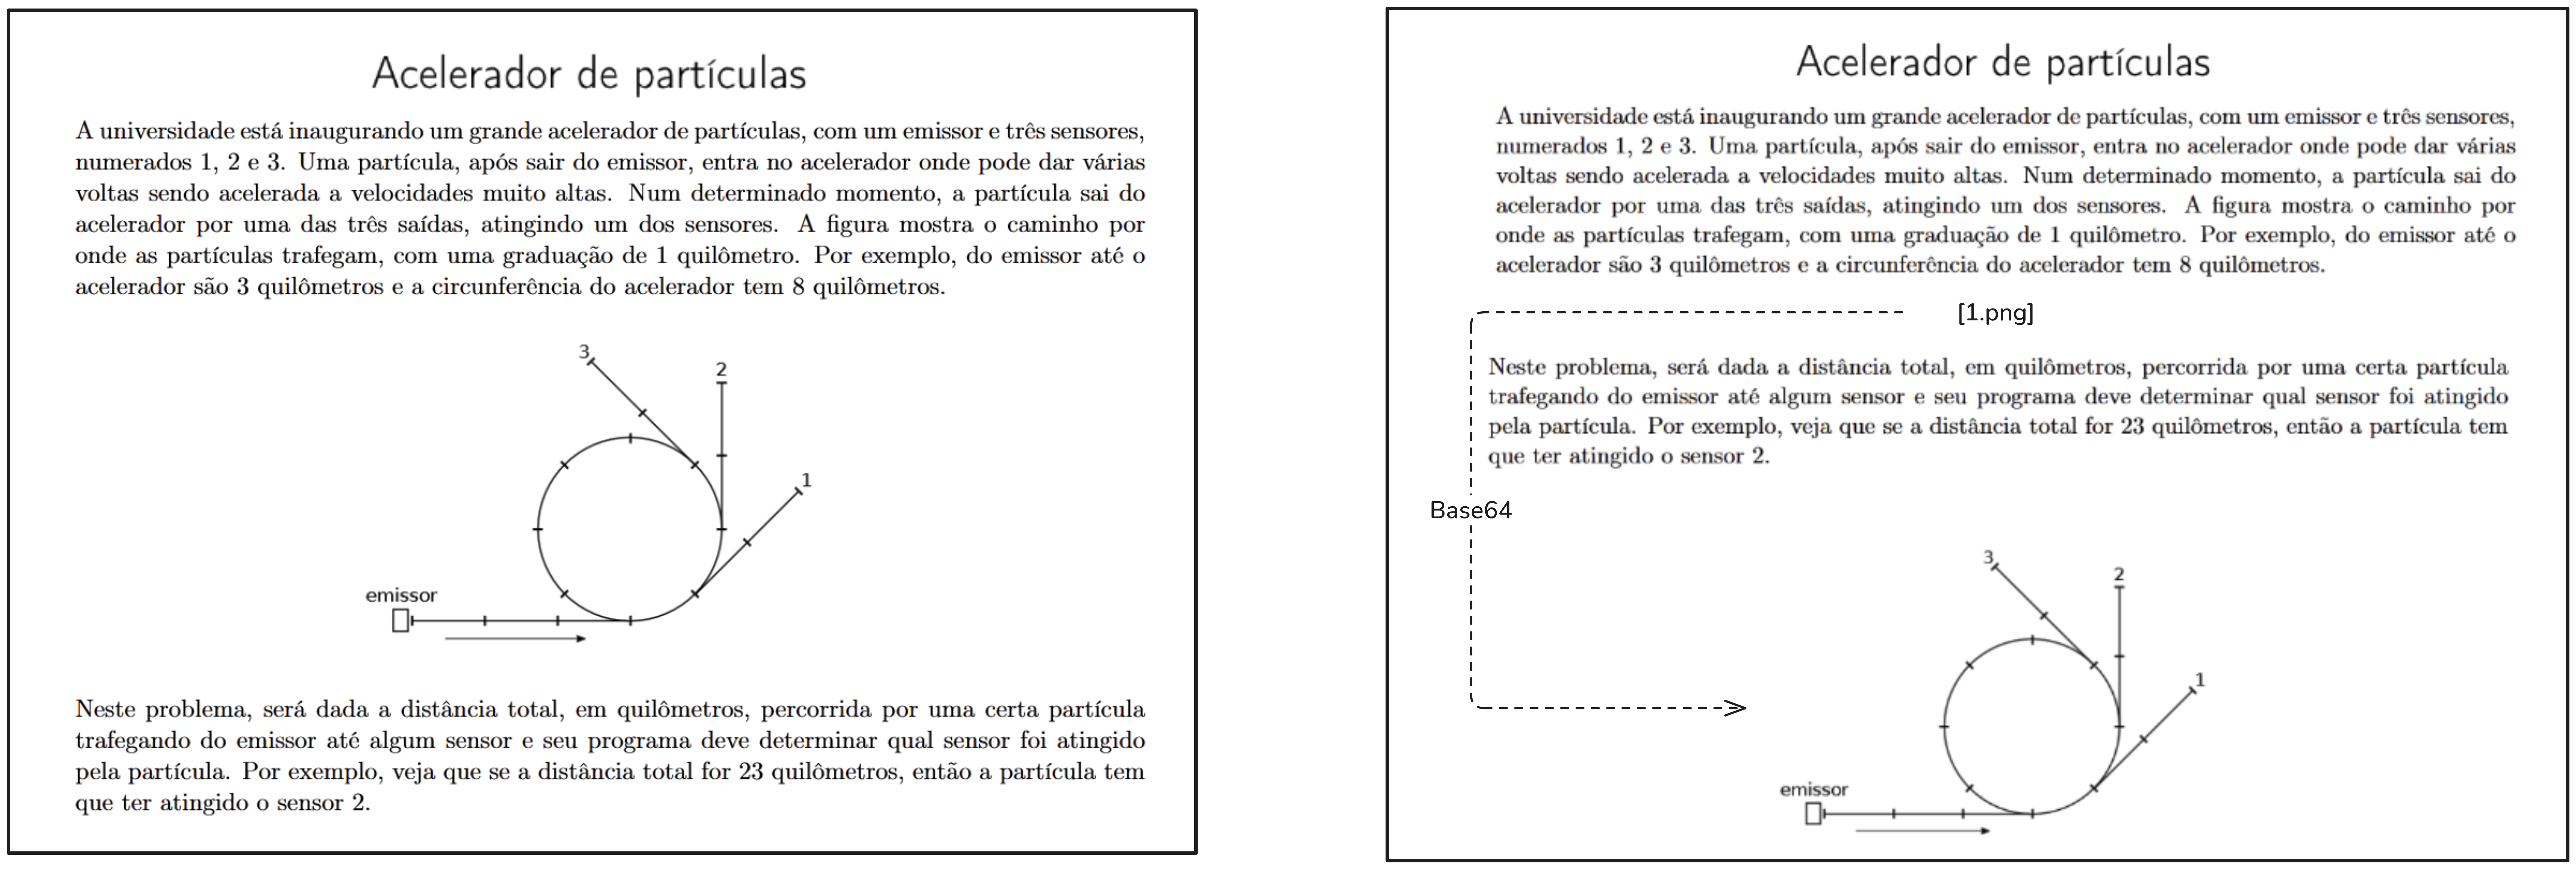
\includegraphics[width=\textwidth]{Cap04/figuras/enunciado-prompt-horizontal.png}
\caption[Representação de um enunciado com imagem no prompt]{Comparação entre o enunciado original da prova da OBI com figura (à esquerda) e a sua representação estruturada no \textit{prompt} com o marcador \texttt{[1.png]} associado à imagem codificada em Base64 (à direita).}
\label{fig:met-enunciado-prompt}
\end{figure}

\subsection{PP3: Explicitação de Limites de Tempo e Memória}\label{sec:met-rq3}

Para isolar o impacto da explicitação das restrições computacionais (\texttt{include\_limits=True}), seleciona-se a linguagem que apresentou a menor taxa agregada de aprovação na PP1 (\linguagem{C}), submetendo novamente todos os 125 problemas com os valores exatos de \texttt{time\_limit} e \texttt{memory\_limit} informados no \textit{prompt} (\promptname{zero\_shot.txt}).

\subsection{PP4: Estratégias de Engenharia de \texorpdfstring{\textit{Prompt}}{Prompt}}\label{sec:met-rq4}

Mantendo \linguagem{C} como linguagem-alvo de maior desafio no \textit{baseline}, comparam-se três estratégias de \textit{prompting} sobre os 125 problemas ($1.125$ execuções ao todo, cujos textos integrais constam do Apêndice~\ref{ap:prompts}): (i) \textit{Zero-Shot} (\promptname{zero\_shot.txt}); (ii) \textit{Few-Shot} (\promptname{few\_shot\_c.txt}), contendo três problemas canônicos em C voltados à prevenção de \textit{overflow}, E/S estrita e indexação 1-based; e (iii) \textit{Chain-of-Thought}~\citep{wei2022chain} guiado pela Metodologia de Pólya~\citep{polya1945} (\promptname{chain\_of\_thought\_polya.txt}), estruturado em Compreensão, Planejamento, Codificação (Execução) e Teste. Adicionalmente, conduz-se uma auditoria manual e programática (\textit{sanity check}) sobre os casos classificados como \veredito{CE} no \textit{CoT Pólya} para verificar se contêm código C compilável suprimido por artefatos de extração de múltiplos blocos Markdown (\textit{parser artifact}).

\subsection{PP5: Evolução Geracional sob Paridade de Juiz}\label{sec:met-rq5}

Para avaliar o progresso entre gerações consecutivas de LLMs sem introduzir distorções de protocolo, identificou-se a interseção exata entre a base Sênior deste TCC e o estudo preliminar do grupo~\citep{angelo2026ise,obibenchmarking2026}. Esse recorte corresponde à totalidade das \textbf{46 questões com figuras} do Nível Sênior da OBI (2016--2025), único subconjunto compartilhado que dispõe de execuções sob configuração idêntica em ambos os trabalhos: linguagem \linguagem{Python}, estratégia \textit{Zero-Shot}, modo texto puro (\modalidade{text}) e decodificação determinística ($T = 0{,}0$).

Uma etapa metodológica decisiva consistiu em \textbf{rejulgar localmente os códigos \texttt{.py} salvos da geração anterior} (\textbf{Gemini 3.1 Pro} e \textbf{GPT-5.4}) utilizando exatamente o mesmo \texttt{JudgeService} empregado para \textbf{Gemini 3.8 Flash} e \textbf{GPT-6 Luna}. No repositório anterior, o avaliador aplicava tempo limite fixo de $3{,}0\,\mathrm{s}$ para \linguagem{Python} (independentemente do limite oficial de $5{,}0\,\mathrm{s}$ previsto em diversas questões da OBI) e comparava saídas com remoção de espaços apenas nas extremidades da \textit{string} completa, em vez de linha a linha. Sem o rejulgamento no ambiente unificado (Python~3.14.3, limites oficiais por questão e monitoramento de memória via \texttt{psutil}), diferenças de infraestrutura seriam confundidas com ganhos ou perdas reais dos modelos.

Os resultados consolidados desse protocolo foram organizados no arquivo \href{https://github.com/mestrevh/competitive-programming-bench/blob/main/results/dataset_obi_senior/llms_compare.csv}{\texttt{results/dataset\_obi\_senior/llms\_compare.csv}}\footnote{Disponível em: \url{https://github.com/mestrevh/competitive-programming-bench/blob/main/results/dataset_obi_senior/llms_compare.csv}.}. Para preservar a simetria da análise pareada entre gerações, a avaliação na PP5 restringe-se às famílias com cobertura completa nos dois ciclos --- \textbf{Google} (\textit{Gemini 3.1 Pro} $\rightarrow$ \textit{Gemini 3.8 Flash}) e \textbf{OpenAI} (\textit{GPT-5.4} $\rightarrow$ \textit{GPT-6 Luna}). A família DeepSeek não entra nas tabelas e nos gráficos comparativos dessa seção porque o antecessor \textit{DeepSeek-V3.2} não possui execuções \linguagem{Python} \textit{Zero-Shot} no Nível Sênior, permanecendo registrado como \texttt{N/A} na base consolidada.

\section{Limitações}\label{sec:conc-limitacoes}

Embora o protocolo experimental tenha sido estruturado para garantir controle e reprodutibilidade, algumas limitações metodológicas devem ser consideradas. Primeiramente, a avaliação concentra-se na geração determinística ($T = 0{,}0$) com a métrica $\passat{1}$ (uma única submissão por problema e condição), diferindo de estudos que variam o parâmetro $k$ com temperaturas mais altas para explorar a diversidade amostral dos modelos.

Além disso, o escopo empírico principal restringe-se a três modelos atuais e às questões do Nível Sênior da OBI, enquanto a comparação geracional (PP5) limita-se à interseção de 46 questões com figuras em \linguagem{Python} \textit{Zero-Shot} e aos dois pares com cobertura completa (Google e OpenAI). Como os problemas correspondem a edições públicas aplicadas entre 2016 e 2025, não é possível descartar a hipótese de exposição prévia de parte dos enunciados ou soluções nos conjuntos de treinamento dos modelos. Por fim, o extrator automático de código apresenta sensibilidade a respostas que dividem a solução em múltiplos blocos Markdown, aspecto que motivou a auditoria específica de artefatos de extração na PP4.